\begin{appendices}

    \chapter{Entity Relationship (ER) diagram for RDBMS} \label{ch:appendix_rdbms}

        The Entity Relationship (ER) diagram for the PostgreSQL database that was implemented as a part of this thesis is presented on the following page.
        In this database, Teranet dataset augmented with new features and land use produced by the best-performing classification algorithm is combined with related Census and TTS tables.
        Referential integrity constraints of this database were set up to reflect the nature of the spatial and temporal relationships introduced in chapter~\ref{ch:spatial_and_temporal_relationships}}.

        \begin{figure}[hbt!]
            \centering
            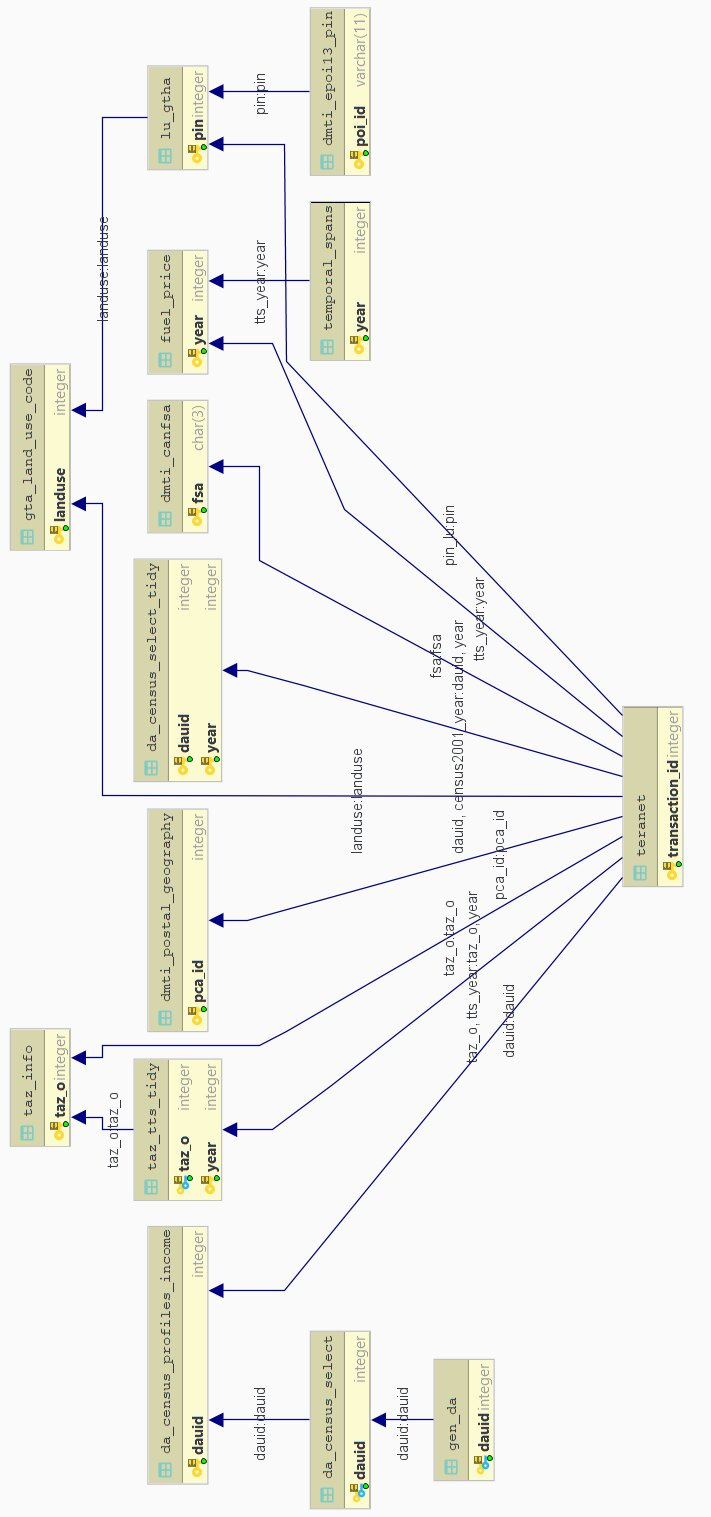
\includegraphics[width=0.65\linewidth,trim=0 0 0 0,clip]{db_schema_vert.jpg}
            \caption{Entity Relationship (ER) diagram for the PostgreSQL database that was implemented as a part of this thesis.
            In this database, Teranet dataset augmented with new features and land use produced by the best-performing classification algorithm is combined with related Census and TTS tables.
            Referential integrity constraints were set up to reflect the nature of the spatial and temporal relationships introduced in chapter~\ref{ch:spatial_and_temporal_relationships}}.
            \label{fig:db_schema_vert}
        \end{figure}

    \end{appendices}
